\documentclass[a4paper, 11pt]{article}

%\usepackage[swedish]{babel}
%\usepackage[TI]{fontenc}
%\usepackage[latin1]{inputenc}

% For setting up margins in the document
\usepackage[left=3.5cm, right=3.5cm, top=3.5cm]{geometry}
\usepackage{comment}

% Code formatting when using lstlistings
\usepackage{color}
\definecolor{code_keywords}   {rgb}{0.13,0.13,0.75} %blue={0.13,0.13,0.75}
\definecolor{code_comments}   {rgb}{0.17,0.57,0.17}
\definecolor{code_linenumbers}{rgb}{0.5,0.5,0.5}
\definecolor{code_strings}    {rgb}{0.5,0,0} %red={0.5,0,0}
\usepackage{listings}
\lstset{
	inputpath        = code,
	% language		 = Python,
	language		 = C,
	basicstyle		 = \footnotesize \ttfamily,
	commentstyle	 = \color{code_comments},
	keywordstyle	 = \bfseries\color{code_keywords},
	stringstyle		 = \color{code_strings},
	%numberstyle		 = \tiny\color{code_linenumbers},
	%frame			 = l,
	keepspaces		 = true,
	%numbers			 = left,
	%numbersep		 = 5pt,
	showspaces		 = false,
	showstringspaces = false,
	showtabs		 = false,
	stepnumber		 = 1,
	tabsize			 = 4,
}

\usepackage{graphicx} % For figures

\usepackage{comment} % For multiline comments

\usepackage{enumitem}

\usepackage{amsmath}

\usepackage{hyperref}

\usepackage{subcaption}

\title{A TS Calculator for 3D models}
\author{John Daniel Bossér and Lennart Bossér}

\newcommand{\TS}{\mathrm{TS}}

\begin{document}

\begin{comment}
    % For figures
    \begin{figure}
        \centering
        \includegraphics[width=0.5\textwidth]{}
        \caption{}
    \end{figure}

    % For lists with a), b), c) etc. 
    \begin{enumerate}[label=\textbf{\alph*)}]
        \item 
    \end{enumerate}
    
    % For code
    \begin{lstlisting}     
    Code goes here
    \end{lstlisting}


\end{comment}

\maketitle

\section{Introduction}

    \begin{figure}
        \centering
        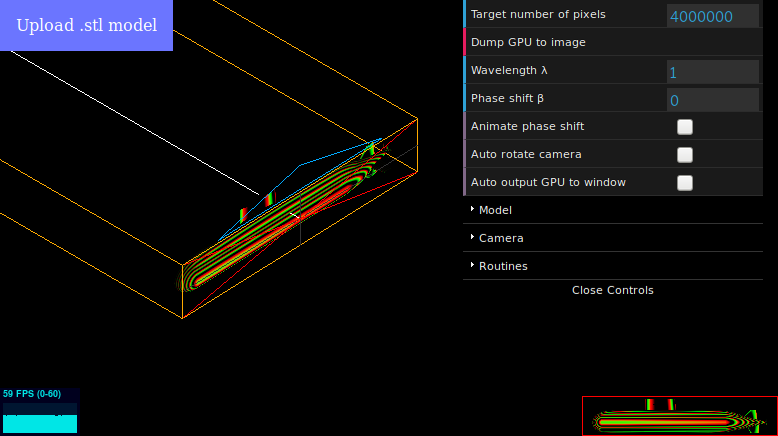
\includegraphics[width=0.9\textwidth]{figures/screenshot.png}     
        \caption{The program}
        \label{fig:screenshot}
    \end{figure}

    The purpose of this program is to calculate the monostatic target strength (TS) for any 3D model quickly by using the graphics pipeline. This program was written in Javascript and relies on Three.js\footnote{\url{https://threejs.org/}} as an interface to WebGL. WebGL is then used for parallel computation of sound reflection of an incoming plane sonar wave in the monostatic case. A screenshot of the program in question can be seen in figure \ref{fig:screenshot}.
        
\section{Theory and idea}

    The TS can be calculated as 
    \begin{align}
        \label{eq:raw_TS}
        \TS = 20 \log \left|\int_S \frac{\cos(\theta)}{\lambda} e^{-2kr} dS \right|
    \end{align}
    where $S$ is the projected surface of the model on the plane normal to the incoming sonar wave, $\theta$ is the angle between the incoming wave and surface normal, $\lambda$ is the wavelength, $r$ is the distance from the sonar to local surface center, $k = 2\pi/\lambda$ and $dS$ is the surface element of the projected surface. The main idea of the program is to discretize equation \ref{eq:raw_TS} as  
    \begin{align}
        \label{eq:disc_TS}
        \TS & \approx 20 \log \left| \sum_S \frac{\cos(\theta)}{\lambda}e^{-2kr} \delta S \right| \\ 
            & \approx 10 \log \left| \frac{\delta S}{\lambda} \sum_S \cos(\theta) \cdot [\cos(-2kr) + i\sin(-2kr)] \right|^2  \\
            & \approx 10 \log \left[ \frac{\delta S}{\lambda} \left( \sum_S \cos(\theta)\cos(-2kr)  \right)^2 + \frac{\delta S}{\lambda}\left( \sum_S \cos(\theta)\sin(-2kr)  \right)^2  \right] 
    \end{align}
    where $S$ is now subdivided into a grid each with an area of $\delta S$. By letting $\delta S$ be the part of the model that corresponds one pixel of the model, one can use the graphics pipeline to calculate $\cos(\theta) \cos(-2kr)$ and $\cos(\theta) \sin(-2kr)$ at every $\delta S$ element by calculating them as the colors of the pixel.
    
    In practice, this is done by implementing a fragment shader; a program run on the GPU responsible for coloring each pixel of the model. The fragment shader is written in GLSL\footnote{\url{https://www.khronos.org/opengl/wiki/Core_Language_(GLSL)}} and calculates $\cos(\theta) \cos(-2kr)$ and $\cos(\theta) \sin(-2kr)$ and places the the values in the green and red channel respectively. The CPU then reads the output image and evaluates the sum and multiplication operations in equation (\ref{eq:disc_TS}).  

\section{Tests of validity}

    The software was tested by measuring the TS as a function of frequency for a plane wave hitting a stiff sphere with a radius of 2 meters. The results of this can be found in figure \ref{fig:sphere_test}. From the pictures, we can see that this program computes the correct TS for a wide range of frequencies in the optics region, and that this range can be increased by increasing the resolution of the images. 
    \begin{figure}
        \centering
        \begin{subfigure}{0.45\textwidth}
            \includegraphics[width=\linewidth]{figures/spheretest1.png}
        \end{subfigure}
        \begin{subfigure}{0.45\textwidth}
            \includegraphics[width=\linewidth]{figures/spheretest2.png}
        \end{subfigure}
        \caption{TS as a function of frequency for a stiff sphere with a 2-meter radius. The two different images show the calculations for two different resolutions. The left image is calculated using a 200x200 resolution, while the right image uses a resolution of 2000x2000. We can see that the calculations become unstable for higher frequencies and that the calculations are stable for a wider range of frequencies when using a higher resolution. We can also see that the program gives the correct TS for a wide range of frequencies in the optics region.}
        \label{fig:sphere_test}
    \end{figure} 

\section{Implementation}
    
    % Write about 

    \subsection{The vertex shader}
        
        % The vertex shader
        Before the pixel values can be colored the model is first fed through the vertex shader. This shader is responsible for modifying the mesh of the model. This is not of much interest for this application. However, a simple vertex shader needs to be implemented to feed-forward information to the fragment shader about the coordinates of the model (used to calculate $r$) and vertex normals (used to calculate $\cos(\theta)$). This is done by declaring \textit{varying} variables that provide an interface between the vertex shader and the fragment shader. 

    \subsection{The fragment shader}
        
        % The fragment shader
        Each pixel of the model is colored using the fragment shader. Here, we calculate the angle between the incoming sound wave direction and the surface normals using the dot product. This gives $\cos(\theta)$. We also take the dot product between the incoming sound wave direction and the model coordinates to get $r$. The values $\cos(\theta)\cos(-2kr)$ and $\cos(\theta)\sin(-2kr)$ are then written to the red and green channels. 
    
    % The computation camera
    \subsection{The computation camera}
        
        Imagine the case where a large part of the model is outside the rendering view. In that case, we would make a lot of useless computations on black pixels and the sum in equation (\ref{eq:disc_TS}) would not be computed on the whole surface. To solve these problems, we use an extra camera which purpose is to capture the whole model while minimizing the unused black pixels. Whenever the model is rotated the cameras aspect ratio is modified and is translated in space to always have an optimal view of the model. 

        The source of the sound is coming from behind the camera. Thus, this camera is effectively the receiver of the reflected sound on this monostatic setup. 
     
\section{Further work}

    \subsection{Optimization}
        
        \subsubsection{Extracting the four channels}
        The calculated data values taken from the GPU consists of one array consisting of four channels: red, green, blue and alpha. When these values are retrieved from the GPU they come in a list with a structure like $[r_0, g_0, b_0, a_0, r_1, g_1, b_1, a_1, \dots, r_N, g_N, b_N, a_N]$, where $N$ is the number of pixels in the image. Currently, the solution to extract the four different channels is by iterating over the list using a \lstinline{for}-loop. This is though inefficient in two ways. First, letting the CPU iterate over each pixel is of course not a suitable task for the CPU. As an improvement one should look into if it is possible for the GPU to either output into four lists immediately or rendering each channel one at a time. Secondly, the Javascript \lstinline{for}-loops are executed imperatively, and should nowadays be replaced by \lstinline{Array} functions such as \lstinline{map}, \lstinline{filter} and \lstinline{reduce} since these functions are further optimized. The second approach should be considered if the first approach is not feasible.  

        \subsubsection{Fitting the computation camera to the model}
        The camera used for computation tries to minimize the black area around the image while still fitting the entire model in the view. However, this turned out to be a difficult problem to solve, and is arguably still not solved. There are times when the model are slightly out of frame, and there is still a black area around the model. Due to time limitations, this was only partially fixed and should be improved when writing a more production-ready application. 
        
    \subsection{Suggestions for further work}
        
        \subsubsection{.obj model files and layers in the model}
        Since this program can only really examine shells of 3D models consisting of fully reflective materials, one should look into extending the program to work with .obj model files. In the programs current form it can only import STL models. .obj files have the advantage that the model can consist of different materials that can be assigned different aucoustical properties. Furthermore, one could then also look into performing computations on more layers of the model to see the interaction effect of the reflected sound which occur when the reflection of the inner parts of the model and shell interact.  

        \subsection{Bistatical analysis}
        This should be rather easy to implement. The two main changes are that the reflected intensity depends on the angle between surface position and camera, as well as the angle of the incoming sound. The phase will accordingly be dependent on both the distance traveled by the sound as well as the distance to the receiver/computation camera.

        \subsection{Point source of sound}
        The incoming sound wave is in its current form a plane wave. One could extend the program to compute phase and intensity from a point source in space. This can be achieved by implementing a new fragment shader. $\cos(\theta)$ would then be calculated as the dot product between the surface normal and the normalized vector of difference between the point source and the surface location in space. 

        \subsection{Summation on GPU}
        One bottleneck in the program is the evaluation of the sums in equation (\ref{eq:disc_TS}) since the CPU needs to traverse every pixel one by one to calculate the sum. Potentially this could be sped up using routines on the GPU. 

        \subsection{Summation using Numpy}
        If one cannot implement the summation on the GPU, one could look into writing a summation script in Numpy and exposing it to this Javascript application through a server. The main benefit of this would be the use of the highly optimized routines implemented in C and FORTRAN that are much faster compared to ordinary Javascript. 
        
        \subsection{Other use cases}
        One should also look into trying to either apply this application or extend it to deal with other problems from physics. One potential area of interest would be in electrodynamical applications since many of these problems also involve surface integrals that can be quickly computed using the power of the GPU. 


\end{document}
